\chapter{Other Factors and Future Work}

\section{Evidence of Other Influencing Factors}
\label{sec:otherfactors}

In the following example, the same anchor set is used in four different random networks.  Figure~\ref{fig:AS6good} shows two non-outlier cases.  The mean error for each network, despite using the same anchor set, is different.  What is surprising is the degree to which they are different: 37\%.  Further, Figure~\ref{fig:AS6bad} shows two more networks with the same anchor set.  This time, both of the plots reveal outlier cases.  While we have shown that anchor placement does play a role in the localization performance, this simple example clearly shows that there are significant other factors affecting the localization error.

\begin{figure}
  \centering
	\subfloat[Network A]{\label{fig:AS6NetworkDiff7}
		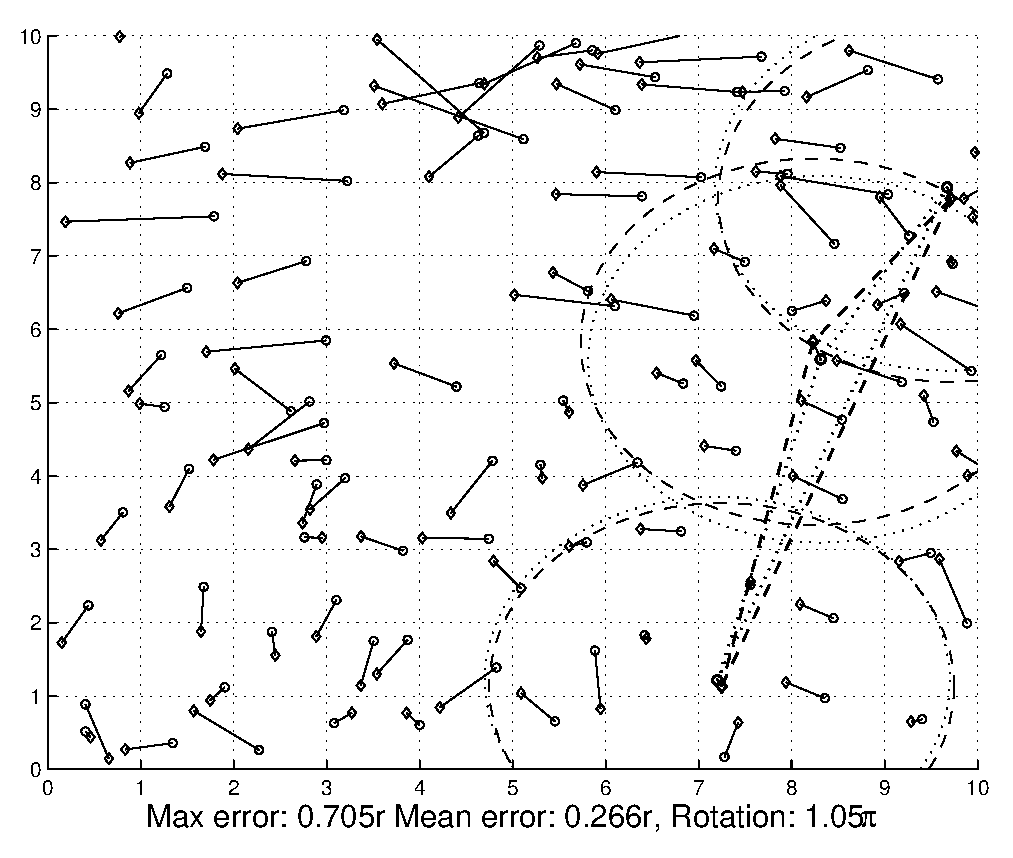
\includegraphics[width=\figurewidth\textwidth]{outliers/AS6/AS6NetworkDiff7}}
	\\
	\subfloat[Network B]{\label{fig:AS6NetworkDiff10}
		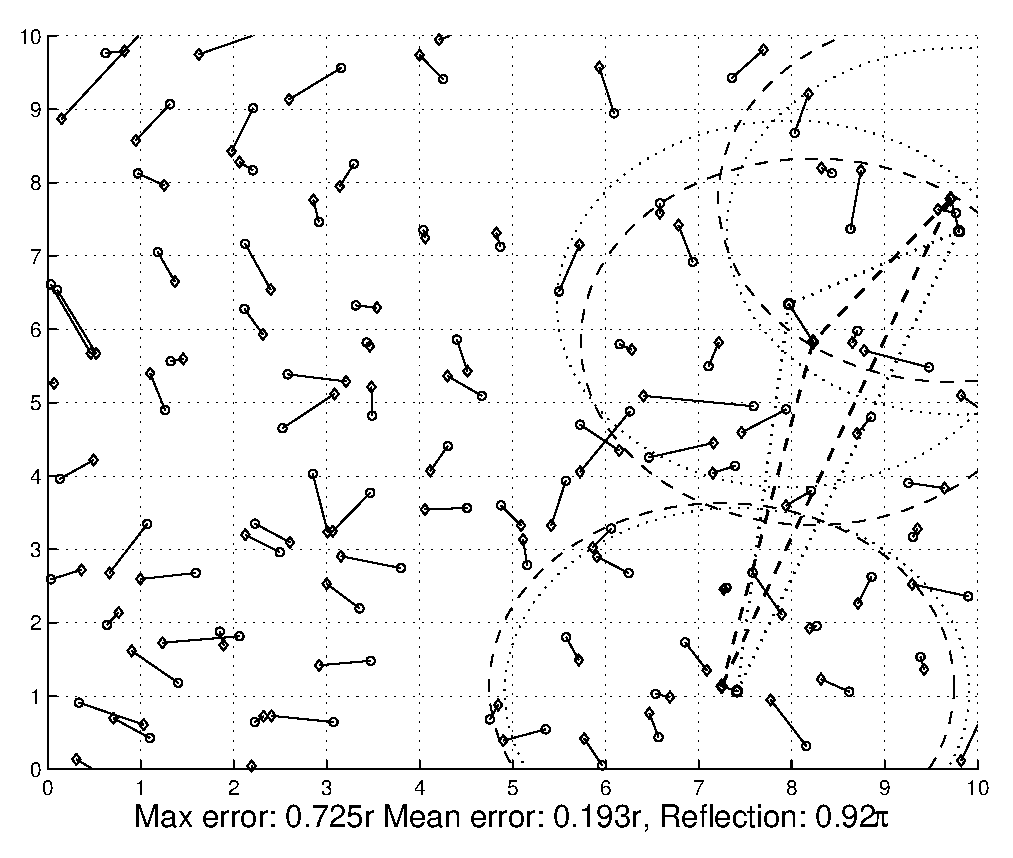
\includegraphics[width=\figurewidth\textwidth]{outliers/AS6/AS6NetworkDiff10}}
	\caption{Good localization performance with same anchor set in two different networks}
	\label{fig:AS6good}
\end{figure}

Further, Figures~\ref{fig:AS6bad1} and \ref{fig:AS6bad2} show two more random networks, using the same anchor set as above.  As seen in Chapter~\ref{chap:outliers}, some short anchor node triangles can cause extremely poor localization.  In this case, we see that even the same anchor set does not necessarily mean that the resulting localization results will be so poor.  

\begin{figure}
  \centering
	\subfloat[Network C]{\label{fig:AS6NetworkDiff9}
		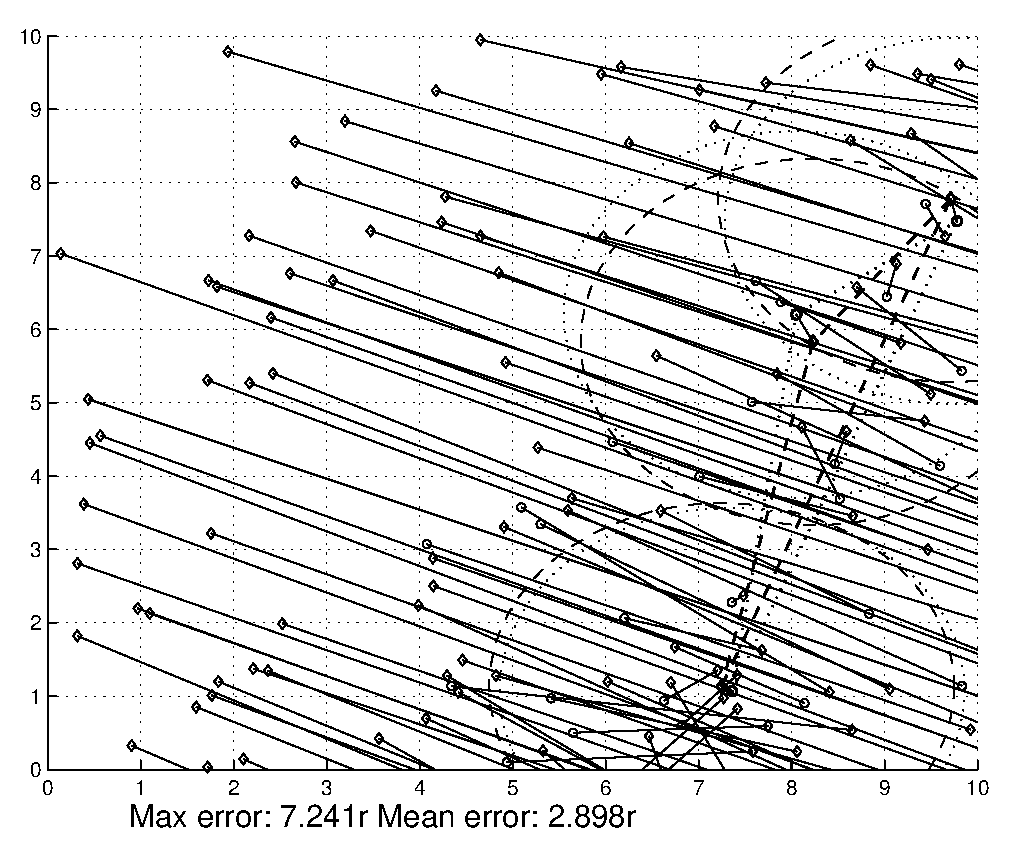
\includegraphics[width=\figurewidth\textwidth]{outliers/AS6/AS6NetworkDiff9}}
\\
	\subfloat[Network D]{\label{fig:AS6NetworkDiff8}
		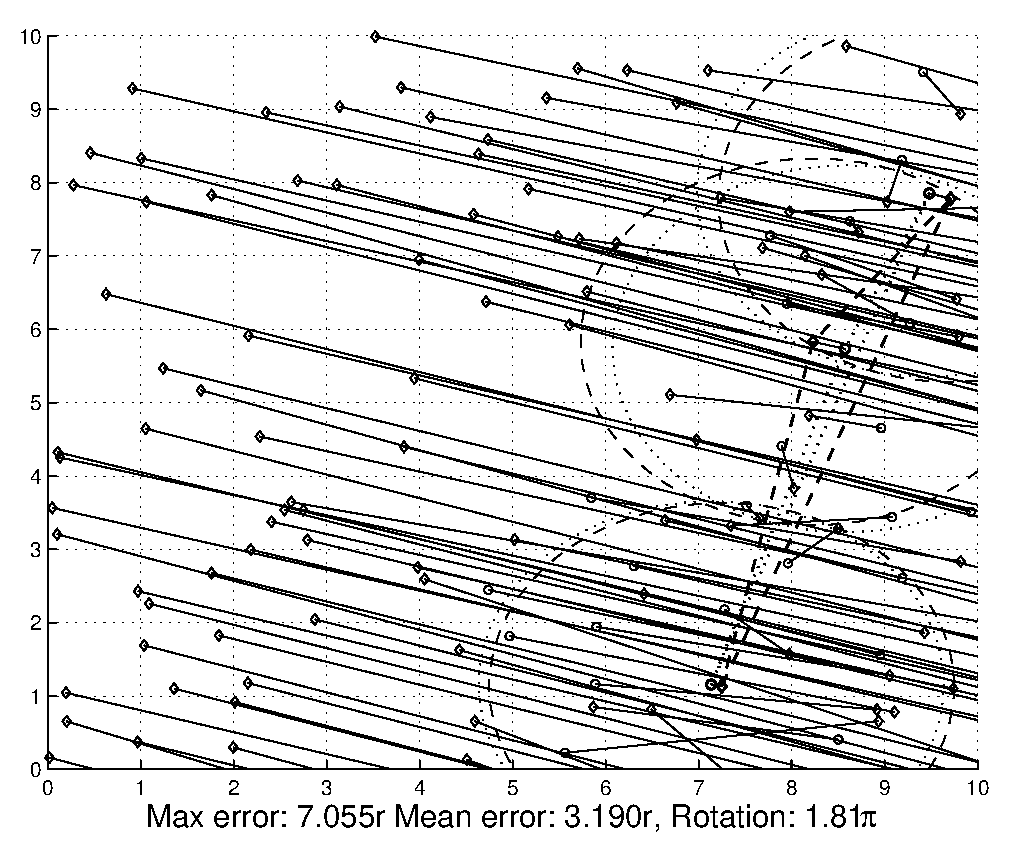
\includegraphics[width=\figurewidth\textwidth]{outliers/AS6/AS6NetworkDiff8}}	
    \caption{Poor localization performance with same anchor set in two different networks}
	\label{fig:AS6bad}
\end{figure}

Based on these results, there is clearly some other factors besides anchor placement effecting the resulting location errors.   However, since the outlier case itself is undetectable in the absence of extensive ground truth data, the best we can hope for is a way to minimize the probability beyond analyzing the height of the anchor node triangle by studying what these other factors might be.  These factors might include network density and the starting node chosen to patch local maps together.

\section{Other Future Work}

